\documentclass{../lab_class}

\usepackage{fancyhdr}
\pagestyle{fancy}
\rhead{П.\,Ю. Смирнов, 687 гр.}
\lhead{Лабораторная работа № 4.2.1, МФТИ, весна 2018}

\begin{document}

{\Large 4.2.1 -- Кольца Ньютона.}

\paragraph{Цель работы.}
Познакомиться с явлением интерференции в тонких плёнках (полосы равной толщины) на примере колец Ньютона и с методикой интерференционных измерений кривизны стеклянной поверхности.

В работе используются: измерительный микроскоп с опак-иллюминатором; плосковыпуклая линза; пластинка из чёрного стекла; ртутная лампа ДРШ; щель; линзы; призма прямого зрения; объектная шкала.

\paragraph{Теоретическая часть.}
\begin{wrapfigure}[12]{r}{5cm}
	\centering
	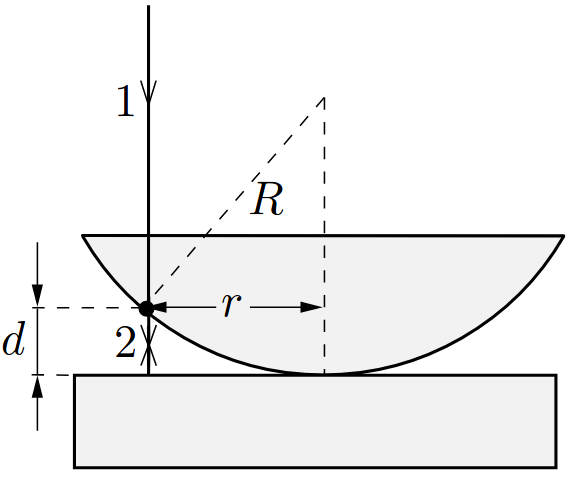
\includegraphics[width=4cm]{sch01.png}
	\caption{Схема наблюдения колец Ньютона}
	\label{pic:01}
\end{wrapfigure}

Классический опыт Ньютона можно использовать для определения радиуса кривизны сферических пластин. В этом опыте свет падает нормально на пластину и интерферирует со своим отражением от стеклянной поверхности, на которой лежит линза. Можно пренебречь отклонением луча от нормали при выходе из стекла; тогда (см. рис. 1) при $R \gg d$ имеем $d = r^2 / 2R$. При отражении от оптически более плотной среды свет меняет фазу на $\pi$, отсюда разность хода интерферирующих лучей есть $\Delta = 2d + \lambda/2$. Минимум наблюдается при $\Delta = (2m+1) \lambda/2$, отсюда радиус темных колец
\begin{equation}\label{eq:01}
	r_m = \sqrt{m \lambda R},
\end{equation}
светлых:
\begin{equation}\label{eq:02}
	r_m = \sqrt{(2m-1) m \lambda R/2}.
\end{equation}

Наша нехитрая схема для наблюдения колец изображена на рисунке:
\begin{figure}[H]
\centering
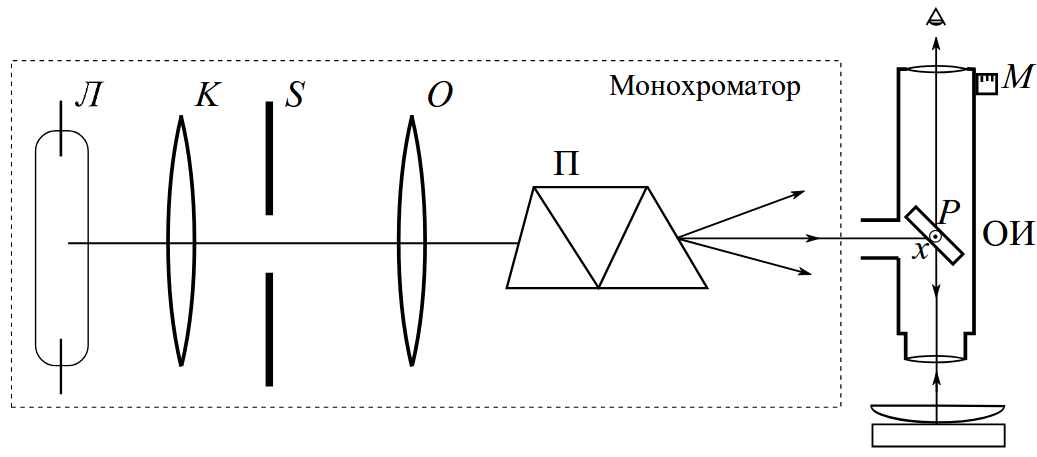
\includegraphics[width = 0.6 \textwidth]{sch02.png}
\caption{Схема установки для наблюдения колец Ньютона}
	\label{fig:scheme}
\end{figure}
Мы используем ртутную лампу с двумя основными спектральными компонентами -- желтой и зеленой. Соотв. интерференционная картина представляет собой периодически чередующиеся участки четкости -- <<биение>>.

\paragraph{Результаты.}

Прямые измерения радиусов колец приведены в таблице. Здесь чередуются последовательно темные и светлые кольца. $m = 1$ -- темное кольцо, $r_1$ следует брать в качестве точки отсчёта. 

\bigskip

\begin{tabular}{|c|c|c|c|c|c|c|c|c|c|c|c|c|}  \hline
$m$  & 1 & 2 & 3 & 4 & 5 & 6 & 7 & 8 & 9 & 10 & 11 & 12 \\ \hline
$r_m$, $\ \smu \m$  & 4.58 & 3.97 & 3.67 & 3.48 & 3.38 & 3.18 & 3.09 & 2.89 & 2.68 & 2.54 & 2.46 & 2.37 \\ \hline
\end{tabular}

\pagebreak
На графике приведены зависимости квадрата радиуса кольца от его номера (с нормировкой на $r_1$). 

\begin{figure}[H]
\centering
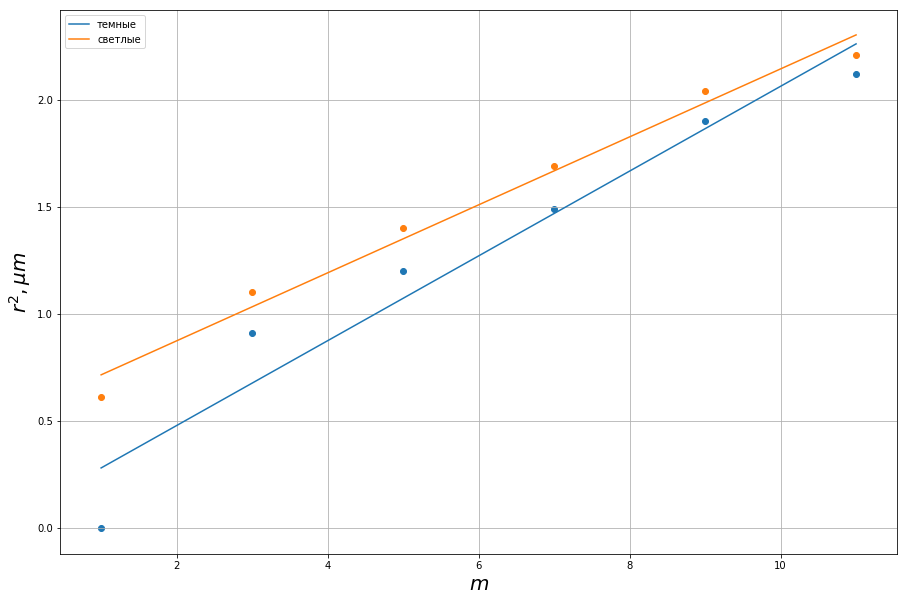
\includegraphics[width = 0.75 \textwidth]{pic.png}
\caption{Квадрат радиуса кольца от его номера}
	\label{fig:main}
\end{figure}

По наклону кривых получаем оценку радиуса кривизны линзы
\begin{gather*}
	R \simeq 1.6 \pm 0.03 \ \m.
\end{gather*}

Размытия нет -- график для темных колец проходит через начало координат. Для биений получаем оценку $\Delta m \simeq 6$, разность длин волн желтой и зеленой компонент ртути -- 33 нанометра.

\paragraph{Вывод.}
Работа демонстрирует полезность использования колец Ньютона для измерения радиуса кривизны линз.

\end{document}